\documentclass[border=5pt]{standalone}
\usepackage{tikz}
\usetikzlibrary{arrows.meta, positioning}
\usepackage{xcolor}

\definecolor{Garnet}{HTML}{73000A}
\definecolor{Atlantic}{HTML}{466A9F}
\definecolor{Horseshoe}{HTML}{65780B}
\definecolor{Honeycomb}{HTML}{A49137}
\definecolor{Rose}{HTML}{CC2E40}

\begin{document}
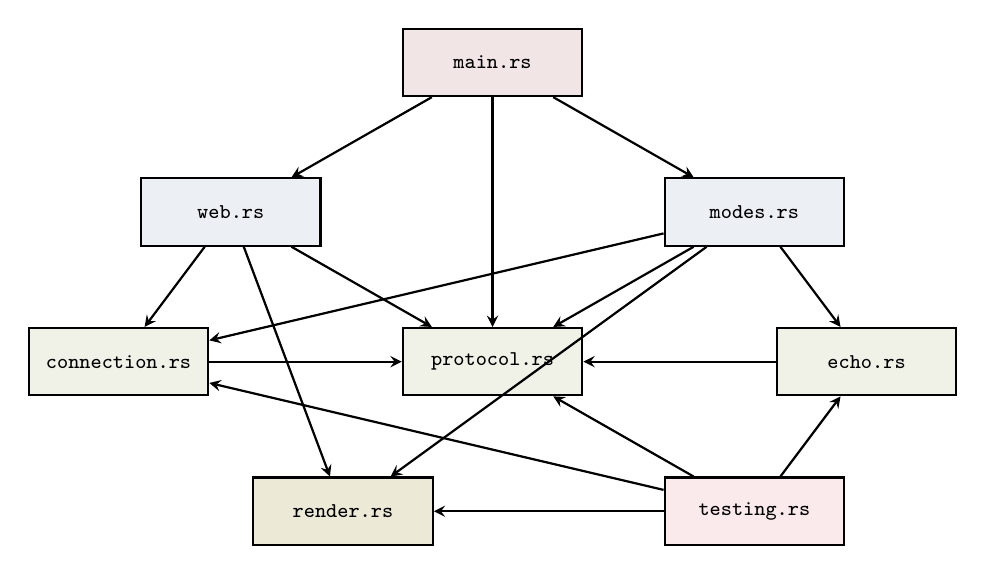
\begin{tikzpicture}[
  mod/.style={draw, thick, minimum width=2.4cm, minimum height=0.9cm, align=center, font=\footnotesize},
  dep/.style={->, thick, >=stealth},
  scale=0.95, transform shape
]
  \node[mod, fill=Garnet!10] (main) at (0,4) {\texttt{main.rs}};
  \node[mod, fill=Atlantic!10] (web) at (-3.5,2) {\texttt{web.rs}};
  \node[mod, fill=Atlantic!10] (modes) at (3.5,2) {\texttt{modes.rs}};
  \node[mod, fill=Horseshoe!10] (conn) at (-5,0) {\texttt{connection.rs}};
  \node[mod, fill=Horseshoe!10] (proto) at (0,0) {\texttt{protocol.rs}};
  \node[mod, fill=Horseshoe!10] (echo) at (5,0) {\texttt{echo.rs}};
  \node[mod, fill=Honeycomb!20] (render) at (-2,-2) {\texttt{render.rs}};
  \node[mod, fill=Rose!10] (testing) at (3.5,-2) {\texttt{testing.rs}};

  \draw[dep] (main) -- (web);
  \draw[dep] (main) -- (modes);
  \draw[dep] (main) -- (proto);
  \draw[dep] (web) -- (conn);
  \draw[dep] (web) -- (proto);
  \draw[dep] (web) -- (render);
  \draw[dep] (modes) -- (conn);
  \draw[dep] (modes) -- (proto);
  \draw[dep] (modes) -- (echo);
  \draw[dep] (modes) -- (render);
  \draw[dep] (conn) -- (proto);
  \draw[dep] (echo) -- (proto);
  \draw[dep] (testing) -- (proto);
  \draw[dep] (testing) -- (conn);
  \draw[dep] (testing) -- (echo);
  \draw[dep] (testing) -- (render);
\end{tikzpicture}
\end{document}
